\chapter[How Cells Hear Outside Messages]{How Cells Hear\protect\\ Outside Messages}

\begin{kaichang}
Your teacher suddenly calls your name. In that second, your heart skips faster, your palms begin sweating, and your face may warm. Think how strange this is: the teacher's voice is merely vibrating air that enters your ears. How does that become a racing heart and working sweat glands? No electrical wire connects your ears to your heart.

Now consider the sensitive plant on the windowsill. A gentle touch makes rows of leaflets close within seconds and the leaf stalk slowly droop as though asleep. Plants have neither nerves nor muscles. How did it hear your touch?

Before reading on, write your guess: what carries the message from ear to heart or fingertip to leaf? By the end, you will see that these seemingly unrelated events share one chemical logic, drawable as a single line of arrows yet coordinating tens of trillions of cells.
\end{kaichang}

\section{Phenomena: A Message Changes Behavior}

Leave molecules aside and consider observable, measurable trigger--response pairs everywhere around you:

\begin{itemize}[itemsep=2pt]
\item Enter a dark room from bright surroundings, and your pupils widen within a second or two. Shine a phone light toward an eye, and the pupil immediately narrows. No decision is needed; it is automatic.
\item Chapter 55's familiar example: blood glucose rises an hour after a meal, then quietly returns to its premeal level two hours later. Something knows glucose is high and orders its recovery.
\item Sprint two hundred meters, and your heart pounds. Rest a few minutes, and it slows on its own. Nobody phones the heart, yet it accelerates and decelerates appropriately.
\item A finger cut becomes red, warm, and slightly swollen: the small surrounding region has received a report that something happened here.
\item Touch makes sensitive-plant leaves close; young shoots on a windowsill bend toward the light outside. Plants also respond to messages, only slowly.
\end{itemize}

Remember three shared features. First, each has a definite \textbf{trigger}: light, sugar, or touch. Second, responses are \textbf{selective}: light constricts a pupil but does nothing to a palm. Cells do not all hear the same message. Third, responses \textbf{subside}: heart rate falls, glucose falls, and sensitive-plant leaves reopen after a dozen or more minutes. Messages must permit finishing as well as starting.

You can observe a response without any reagent.

\begin{shiyan}
\textbf{Watch the Pupil's Automatic Door}

Materials: a small mirror, a flashlight or phone light, and a room that can be darkened.

Procedure: spend two minutes in darkness to adapt. Hold the mirror and briefly direct the flashlight toward your eye from beside your cheek, not straight into the eyeball for a prolonged time, while watching your reflected pupil. Move the light away and observe again. A family member can help by observing from behind and to the side for a clearer view.

Observations: how soon after the light comes on does pupil diameter change, and how fast? How long after removing the light does it recover? Try three brief illuminations: is the third response as large as the first?

Safety: use only brief illumination from an ordinary flashlight. Never use a laser pointer or look directly at the Sun or a bright light source.
\end{shiyan}

\section{Particles: Receptors Are Molecular Doorbells}

Zoom into cells, starting with the sender.

Chemical messages coordinating body parts are carried by \textbf{signaling molecules}. Their sizes vary greatly: the neurotransmitter acetylcholine has a molecular mass just over a hundred; insulin is a small protein of 51 amino acids, as in Chapter 48; histamine, which makes wounds red and swollen, is tiny, with a side chain and a few other atoms. Different sizes and chemical personalities, one job: \textbf{recognition by a particular protein}.

The recognizing protein is a \textbf{receptor}. Chapter 51 described the many membrane-embedded proteins, including receptors spanning the membrane with an outside recognition end and an inside relay end. Recognition is not mysterious. It uses Chapter 48's noncovalent interactions: complementary shapes, charge attraction, hydrogen bonds, and hydrophobic effects. A signal fits a surface pocket and is held by weak interactions, making binding \textbf{reversible}: after a while, it drifts away. Reversibility is essential for a message to end.

The real action follows binding. When the signal enters its pocket, the receptor changes shape slightly, Chapter 48's allostery. This deformation passes from the outside to the inside end, where the chemical environment sees a change. Appreciate the causal chain: \textbf{the receptor understands nothing; its shape simply changes}. A doorbell does not know its visitor; pressing it closes a circuit.

Not every message uses the outside doorbell. Water-soluble signals, such as insulin, adrenaline, and most neurotransmitters, cannot cross a phospholipid bilayer and use membrane receptors. Small hydrophobic signals, such as Chapter 47's steroid hormones, cross directly into cytoplasm or nuclei and bind internal receptors to adjust gene expression. These hand-delivered messages return in Chapter 70's gene switches.

How many receptors are there? A cell may display \textbf{tens to hundreds of thousands} for one signal, while many hormones trigger responses at nanomolar blood concentrations, $10^{-9}$ moles per liter. For scale, $\ud{10^{-9}}{mol}$ is about $6\times10^{14}$ molecules. In a liter of water, that resembles a pinch of salt in a standard swimming pool, yet cells hear it. Such sensitivity comes from what happens next: amplification after the message enters.

\section{Rules: Phosphate Relays Amplify Messages}

The receptor passes the message inside. What relays it there? Nearly all cells use two general mechanisms, often together.

\textbf{First: phosphorylation cascades.} Chapter 50 explained ATP's ability to transfer phosphate groups and change another molecule's reactivity. \textbf{Protein kinases} specialize in attaching ATP phosphate groups to particular sites on target proteins. Adding a phosphate is like pinning on a large badge with two negative charges: local charge and shape change, switching activity on or off, again through allosteric logic. What is attached can be removed: \textbf{phosphatases} remove phosphate groups and reset switches.

The key is that an activated kinase is itself an enzyme, capable of catalyzing repeatedly without being consumed, as Chapter 49 explained. A pathway can therefore form a relay: a receptor activates kinase A, each A activates many B kinases, each B activates many C kinases, and so on. The message amplifies like an avalanche: a \textbf{phosphorylation cascade}.

\textbf{Second: second messengers.} Some activated receptors trigger another membrane enzyme to produce large quantities of a small molecule, such as cyclic AMP, cAMP, roughly an AMP with a changed shape. Others open calcium channels and sharply raise cytoplasmic calcium. Cells normally confine calcium to the ER warehouse in Chapter 57. These small, fast molecules and ions diffuse across cells within milliseconds and broadcast to many downstream proteins. They relay internally after the first messenger, the hormone itself, hence \textbf{second messengers}.

Both mechanisms share an often overlooked default: \textbf{signaling is normally off}. Phosphatases keep removing phosphate, cAMP keeps being degraded, and calcium keeps being pumped into storage. Maintaining on costs continuing energy; stop the message, and everything resets. That is why your heart can slow after speeding up. Reversibility is central, not an incidental benefit.

\begin{qiaoliang}
How much amplification is possible? One adrenaline binds one receptor, which during its active lifetime can activate tens or hundreds of intermediate switch proteins called G proteins. Each activates a cAMP-producing enzyme that can make over a thousand cAMP molecules per second. Each cAMP activates a protein kinase, and each kinase phosphorylates hundreds or thousands of targets. Take conservative numbers: three stages, each amplifying a hundredfold:

\[100\times100\times100 = 10^{6}\]

One signal molecule changes the state of over a million proteins. That is why nanomolar hormone levels can command liver cells to release hundreds of millions of glucose molecules within seconds. The numbers are estimates, but the logic is firm: \textbf{amplification comes not from the signal itself but from Chapter 49's repeated enzymatic catalysis}. The hormone rings once; the house's amplifier supplies the volume.
\end{qiaoliang}

\section{Symbols: A Pathway in One Line}

Now compress the account into symbols. These are \textbf{information-flow arrows}, showing who relays to whom, not Chapter 26's chemical equations for material conversion. One arrow symbol has two meanings; distinguish their contexts.

A typical signaling pathway is:

\[\text{Adrenaline} \rightarrow \text{receptor} \rightarrow \chem{cAMP} \rightarrow \text{protein kinase} \rightarrow \text{target protein} \rightarrow \text{response}\]

Its on and off steps, as material changes, are:

\[\text{Protein} + \chem{ATP} \xrightarrow{\text{protein kinase}} \text{protein--phosphate} + \chem{ADP}\]

\[\text{Protein--phosphate} + \chem{H_2O} \xrightarrow{\text{phosphatase}} \text{protein} + \text{phosphate}\]

A diagram makes the process more immediate:

\begin{center}
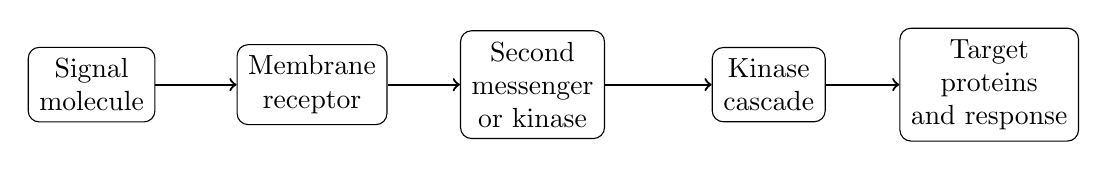
\begin{tikzpicture}[every node/.style={align=center}]
\node[draw, rounded corners, inner sep=4pt] (a) at (0,0) {Signal\\molecule};
\node[draw, rounded corners, inner sep=4pt] (b) at (2.8,0) {Membrane\\receptor};
\node[draw, rounded corners, inner sep=4pt] (c) at (5.6,0) {Second\\messenger\\or kinase};
\node[draw, rounded corners, inner sep=4pt] (d) at (8.6,0) {Kinase\\cascade};
\node[draw, rounded corners, inner sep=4pt] (e) at (11.4,0) {Target\\proteins\\and response};
\draw[->, thick] (a) -- (b);
\draw[->, thick] (b) -- (c);
\draw[->, thick] (c) -- (d);
\draw[->, thick] (d) -- (e);
\end{tikzpicture}
\end{center}

This is related to Chapter 55's metabolic map: that shows \textbf{material} flow, this \textbf{information} flow. A cell lives in both, and the maps interlock: a signaling pathway often ends at a metabolic pathway's switch.

\section{One Doorbell, Different Rooms}

Here is a seemingly contradictory but profound fact: \textbf{the same signaling molecule can produce entirely different responses in different cells}.

Take adrenaline. Being called on, frightened, or starting a sprint makes the adrenal glands release it into blood throughout the body. Heart cells contract faster and harder; liver cells immediately break glycogen down and release glucose as muscle fuel; intestinal smooth muscle instead relaxes and slows digestion, which can wait during an emergency; pupil-dilator muscles widen the pupil to admit more light. One molecule, four contrasting commands, all appropriate.

The secret lies in listeners, not signal. Different cells have \textbf{different receptor subtypes}, like identical doorbells wired to different indoor circuits. Even with the same receptor, intracellular kinase combinations, target proteins, and available gene programs differ. The signal only rings; the occupant's equipment decides the music. Asking what adrenaline does has no single answer: it depends on the cell.

A serious consequence follows: affecting just one body part with a drug is difficult. Asthma drugs widen airways, but similar receptors in the heart make palpitations and tremor common side effects. Blood-pressure drugs block vascular signals but may affect other organs. \textbf{Side effects often mean the same doorbell rang in another room}.

\section{Three Delivery Routes}

Delivery determines how quickly, how far, and how long messages travel. The body mainly uses three routes:

\begin{table}[htbp]
\centering
\begin{tabular}{llll}
\toprule
Route & Typical messenger & Speed and range & Duration \\
\midrule
\shortstack[l]{Endocrine\\(blood broadcast)} & \shortstack[l]{Insulin,\\adrenaline} & \shortstack[l]{Seconds to minutes;\\body-wide} & \shortstack[l]{Longer-lasting;\\fades slowly} \\
\shortstack[l]{Synaptic\\(point-to-point)} & \shortstack[l]{Acetylcholine and\\other transmitters} & \shortstack[l]{Milliseconds;\\next cell only} & \shortstack[l]{Very brief; cleared\\in milliseconds} \\
\shortstack[l]{Paracrine\\(local messages)} & \shortstack[l]{Histamine\\at a wound} & \shortstack[l]{Seconds; within\\a few millimeters} & \shortstack[l]{Local and\\short-range} \\
\bottomrule
\end{tabular}
\end{table}

\textbf{Hormones} use endocrine delivery, secreted into blood and broadcast throughout the body. Only cells bearing the right receptors respond: everyone receives the broadcast, but only those understanding it react. Chapter 55's insulin and glucagon are familiar partners on this route.

\textbf{Neurotransmitters} use synaptic express delivery. The gap between two cells is only about $\ud{20}{nm}$. Transmitter released on one side diffuses across, is received within milliseconds, and is promptly degraded or recovered. Its range reaches just one neighbor and its speed supports piano playing: an ultra-fast, point-to-point version of hormone logic.

\textbf{Local signals} use paracrine delivery. A cut triggers nearby mast cells to release histamine, notifying only a few surrounding millimeters. Blood vessels widen and become slightly leaky so immune cells and repair materials arrive quickly. Redness, swelling, and warmth are the visible effects of this local message.

Plants lack nerves and combine electrical signals with hormones. Ion-generated electrical signals rapidly relay touch in sensitive plants, while slower bending toward light uses uneven auxin distribution across a stem to make one side grow faster. Different routes and envelopes, identical molecular-doorbell response logic.

\section{Feedback, Adaptation, and Noise}

A system that only amplified would soon overload. Signaling includes three reducing mechanisms.

\textbf{Negative feedback:} the response inhibits its own pathway. Chapter 55's metabolic feedback is equally common in signaling: cascade-end products often mute receptors or kinases near the beginning. After blood glucose rises again, insulin secretion and action are suppressed. Feedback makes a self-braking loop instead of a straight accelerator. Body-wide correction of temperature, glucose, and blood pressure amplifies this logic, explored in Chapter 60.

\textbf{Adaptation, or desensitization:} sustained stimulation makes cells turn down the volume. Receptors are phosphorylated and internalized, temporarily removed from display, weakening the response. After a few minutes in a florist's shop, you stop smelling the flowers, not because scent vanishes but because olfactory receptors adapt. Cells become sensitive to change rather than total amount: a changed situation usually deserves more attention than an unchanged one.

\textbf{Noise:} at single-molecule scale, signaling fluctuates intensely. At low hormone concentrations, each receptor encounter is probabilistic; a cell may contain only thousands of a particular kinase, making fluctuations significant. Cells use \textbf{averaging and thresholds}, like reducing noise in photographs: average over time and molecular populations, then require a threshold before responding. Stable macroscopic responses rest on many random microscopic events. From Chapter 9's electron clouds to Chapter 21's thermal motion, statistical averaging overcoming individual fluctuations is a recurring theme.

\begin{zhengju}
If a signal stays outside, how does the inside know? In the 1950s, this puzzled biologists. Adrenaline was known to command liver glycogen breakdown, yet evidence suggested it \textbf{did not enter cells}. How could an outside visitor direct work inside?

The American biochemist Earl Sutherland devised an elegant disassembly experiment. He broke liver cells apart and centrifuged them into membrane fragments and cytoplasm, then tested each separately. Adrenaline added to cytoplasm did nothing; membranes alone also did nothing. But \textbf{recombine the fractions} and add adrenaline, and glycogen-breaking enzymes activated immediately.

The strange result was informative. Adrenaline required membranes, indicating an action there, but membranes must \textbf{produce something diffusible} to carry the message into cytoplasm. Sutherland boiled the mixture, denaturing its proteins, yet the messenger remained active. A heat-resistant small molecule, not a protein, was responsible. Around 1957, he and colleagues identified cAMP.

Alternatives needed exclusion: perhaps adrenaline entered cells and was chemically modified there? Radioactively labeled adrenaline remained almost entirely at the membrane instead of entering. Thus the second-messenger concept emerged: hormone is the first messenger ringing outside; cAMP relays inside. Sutherland received the 1971 Nobel Prize in Physiology or Medicine. Remember the turning point: a result that looked like failure---inactive apart, active together---opened a new concept. \textbf{Apparently failed data often reveal that our categories are wrong}.
\end{zhengju}

\section{Limits: An Averaged Map}

The signal--receptor--cascade--response model is useful, with several boundaries:

\begin{itemize}[itemsep=2pt]
\item Real signaling forms a \textbf{cross-talking network}, not isolated lines. One pathway's intermediates often affect others; textbooks separate chains for clarity.
\item Pathway maps are \textbf{averages of countless measurements}. Individual cells at particular times may deviate from the standard script because molecular populations fluctuate. Here noise returns.
\item Response versus concentration is not all-or-none but a gradually rising S-shaped curve, discussed in the challenge. Whether there is a response really means how strong it is.
\item Lock and key is only a first approximation. Like enzymes in Chapter 49, receptors and signals change shape on binding through induced fit, not rigid insertion.
\item Drug effects vary among people because receptor numbers, metabolic enzymes, age, and health differ. Doses of drugs involving hormones or neurotransmitters must follow medical advice. This chapter explains principles, not medication use.
\end{itemize}

\begin{wuqu}
``More signal means a stronger, longer response, so more supplementation is better.'' This mistakes a doorbell for a volume knob. Adaptation supplies a counterexample: sustained high signal levels promote receptor desensitization and removal, weakening responses. Insulin resistance in type 2 diabetes includes this component: insulin may be plentiful but target cells become less responsive, although the causes are complex and receptor downregulation is only one part. Long-term misuse of external hormones suppresses both the body's secretion and receptor numbers, potentially causing deficiency on stopping. For signaling systems, \textbf{dose and timing are themselves information}. Cells respond to patterns of change, not total molecular tonnage.
\end{wuqu}

\section{Tampered Doorbells: Forged Growth Commands}

Normal cells are disciplined: division requires growth signals, proteins called growth factors that ring matching receptors and initiate division. This is foundational to a multicellular body's order: collective signals, not individual cells, decide when to grow.

Cancer often means \textbf{exploiting the signaling system}, with tricks corresponding to this chapter's parts:

\begin{itemize}[itemsep=2pt]
\item \textbf{A doorbell stuck ringing:} some breast-cancer cells multiply the growth receptor HER2 dozens of times, packing the membrane so densely that the bell effectively stays pressed and growth commands continue.
\item \textbf{A switch stuck on:} the Ras switch protein normally resets after relaying a message. A mutation can prevent resetting and leave it on. About thirty percent of human cancers carry Ras-family mutations, turning a temporary message into a permanent command through one small molecular change.
\item \textbf{Removed brakes:} other proteins stop abnormal signaling or order self-destruction. Their failure leaves cells deaf to stop commands.
\end{itemize}

Notice causality: cancer cells have not become wicked or betrayed the body; cells do not think. Broken molecular switches undermine signaling's statistical logic, and cells follow an altered chemical program.

There is good news within the bad. Knowing which switch is stuck allows molecules to be designed to block it. Imatinib, sold as Gleevec for chronic myeloid leukemia, fits the uncontrolled kinase's pocket and silences it. It transformed a formerly dangerous leukemia into a condition many people can control long term, a milestone in designing drugs from signaling knowledge. Cancer populations can still evolve resistance under drug selection: one switch falls and another mutation rises. This battle is evolution within cell populations, revisited from cooperation and evolution in the next chapter.

\section{Back to the Classroom and Sensitive Plant}

Now fulfill the opening promise. What happens when your name is called?

Sound vibrates cochlear hair cells, mechanically opening membrane ion channels and bringing in Chapter 51's membrane potentials. Electrical signals race along nerves, relayed between stations by neurotransmitters, reaching the adrenal glands. They release adrenaline into the blood's broadcast route. Within seconds it spreads throughout the body: heart-cell receptors activate, cAMP rises, phosphorylation cascades amplify, and the heart beats faster and harder. Sweat glands and skin blood vessels respond through their own receptors and circuits. Racing heart, sweating, and flushing are \textbf{one signal ringing different bells in different rooms}. From vibrating air to faster heartbeat, every unwired gap is crossed by a molecular relay.

The sensitive plant? Touch opens ion channels in pulvinus cells at the leaf-stalk base, spreading an electrical signal. Those cells rapidly release potassium and accompanying water using Chapter 51's pumps and osmosis. Losing water, they soften like deflated balloons, and leaves droop. Later, ions are pumped back, water follows, and leaves rise again. No nerves or muscles, only ions, water, and turgor, yet all four stages remain: ring, relay, respond, reset.

\section{Going Deeper: Listening Cells Build a Cooperative Body}

We have considered how one cell listens. But your body contains tens of trillions: why do some hear a signal and others not? How does the same DNA, identical in every cell, produce contracting muscle cells, electrically active neurons, and hormone-secreting glands? How do cells organize tissues, repair wounds, and yield space when necessary? \textbf{Chapter 59} answers through cellular cooperation. \textbf{Chapter 60} scales signaling's corrections up to homeostasis, continually regulating temperature, glucose, water, and salts. The final signaling destination, receptors entering nuclei to adjust gene switches, takes center stage in Volume III's Chapter 70. You stand at that chain's doorway.

\begin{tiaozhan}
Derive a quantitative concentration--response relation from a simple assumption: ligand \chem{L} and receptor \chem{R} bind reversibly, \chem{L} + \chem{R} $\rightleftharpoons$ \chem{LR}, with dissociation constant $K_d$. The occupied fraction $\theta$ satisfies

\[\theta = \frac{[\chem{L}]}{K_d + [\chem{L}]}\]

When $[\chem{L}] = K_d$, $\theta = 1/2$, so $K_d$ is the concentration for half-occupancy and measures affinity: smaller $K_d$ means greater sensitivity. Plotted against logarithmic concentration, the curve is S-shaped; a tenfold concentration rise moves the response only partway. This explains low-concentration hormone effects and why drug effects cannot grow indefinitely with dose: receptors saturate, and $\theta$ cannot exceed 1. Cooperation among receptors and cascade amplification can steepen the curve and produce threshold responses. Skipping this box does not affect the main argument.
\end{tiaozhan}

\section*{Practice}

\begin{sikaoti}
\item Draw an information-flow map from a teacher calling your name to faster heartbeat. Identify each carrier: sound waves, electrical signals, or a particular molecule. Mark the broadcast and express-delivery sections.
\item A signal initiates three stages, each amplifying a hundredfold. How many target proteins change state? What if each stage amplifies tenfold? Use the comparison to explain what stage count means for amplification.
\item Why does Sutherland's inactive-apart, active-together result strongly suggest a diffusible small messenger? What would be expected if the membrane itself were the messenger?
\item Plot time against cellular response to a continuously applied signal of fixed concentration. Explain the shape using receptor desensitization.
\item A mutation leaves a protein kinase permanently active \textbf{without} a signal. Predict the cell's behavior and possible consequences if the pathway controls division.
\item Asthma drugs act on airway smooth-muscle receptors but often cause palpitations and tremor. Use the same-doorbell/different-rooms idea to explain why side effects are difficult to avoid completely.
\end{sikaoti}
